General-purpose computing on graphics processors (GPGPU) is the use of a graphics processing unit (GPU) to perform computation that would traditionally be performed on the central processing unit (CPU). The majority of GPUs today are programmable using APIs such as OpenCL and CUDA.\@ Using these APIs, applications can utilize GPUs as coprocessors to execute parts of the application.

GPUs are particularly well-suited for problems that can be expressed as data-parallel computations, which is executing the same program on many data elements in parallel, ideally with high arithmetic intensity. Arithmetic intensity is the ratio of arithmetic operations to memory operations. Graphics processing is the original application, but GPUs have found widespread application in other areas such as machine learning.

This chapter focuses on the architecture of NVIDIA GPUs and the CUDA API \cite{nvidia2019cuda}. The alternative would be OpenCL, which is an open API available on hardware from other vendors, which can also run on other types of hardware. CUDA was chosen due to its widespread use, the quality of its documentation as well as the clear relation between the API and the graphics hardware.

\section{GPU architecture}

GPUs have some significant architectural differences to CPUs, something programmers must be aware of to fully utilize the capabilities of GPUs. The architecture of CPUs is designed for a variety of applications, while the architecture of GPUs is designed primarily for graphics applications. The main differences are that GPU memory is divided into multiple regions with different capacities, bandwidths, latencies and access methods, threads on a GPU can communicate in a number of specialized ways and branching instructions are carried out very differently from CPUs.

GPU architectures evolve over time, which exposes new features to programs and influences the way programs must be designed to optimally utilize the available resources. The features of the GPU architecture are expressed as the compute capability which is a string consisting of a major and minor version number, which at the time of writing ranges from 1.x to 7.x. This chapter describes devices with compute capability 6.x and 7.x, which is available in the most recent generations of hardware at the time of writing.

\begin{figure}[h]
    \centering
    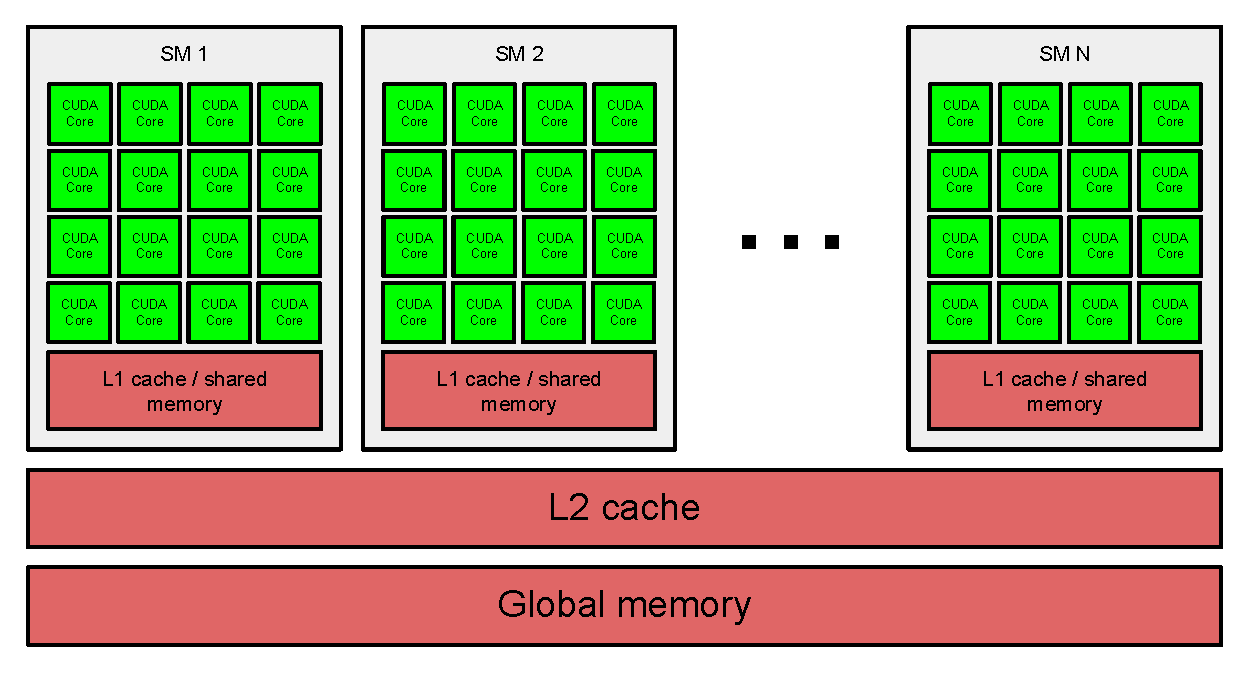
\includegraphics[scale=0.5]{gpu_architecture}
    \caption{Simplified GPU architecture}
    \label{fig:gpu_architecture}
\end{figure}

Unlike the CPU, the GPU dedicates most of its resources to data processing instead of caches and control flow mechanisms. Therefore, the cost of memory accesses and branching is high compared to the cost of data processing such as arithmetic operations. This means that programs with high arithmetic intensity are favored. The individual performance of each thread on a GPU is much lower than the performance of a thread on a CPU, but the GPU makes up for it with the sheer amount of threads that it can execute in parallel.

A GPU contains an array of Streaming Multiprocessors (SMs) and a large shared global memory. The multiprocessors can access the global memory and have an L2 cache that is shared by all multiprocessors. Each multiprocessor has its own L1 cache and on-chip memory that is only accessible to the multiprocessor. The GPU and CPU are connected through an interface such as PCI-e. The bandwidth of the global memory is much higher than the bandwidth between the GPU and CPU.\@ Similarly, the bandwidth of the on-chip memory is much higher than the bandwidth of the global memory.

\subsection{SIMT architecture}

Work is carried out by creating groups of threads to run a program, and distributing threads between the multiprocessors in groups of 32 parallel threads called warps. A group of warps may have interdependent threads and must be scheduled onto the same multiprocessor. Each multiprocessor creates, manages, schedules and executes threads in warps. A warp is the smallest unit of execution, meaning that instantiating a number of threads that is not divisible into warps requires leaving a remainder of threads unutilized. All threads in a warp share a single program but have their own program counters and register states. Warps execute independently, but may share a program and shared memory with other warps in the same multiprocessor, and may also share a program and global memory with warps on other multiprocessors.

Within the multiprocessors, warps are executed with a Single Instruction, Multiple Thread (SIMT) architecture, meaning a warp executes one common instruction at a time on all 32 threads in parallel. Full efficiency is realized when all 32 threads have non-divergent execution paths. When the execution paths diverge, the warp can execute only the common instruction of one subgroup of threads at a time by disabling non-participating threads. Because warps execute independently, the effects of branch divergence only happen within a warp.

The execution of warps within a multiprocessor is efficiently interleaved by warp schedulers, so that another instruction can be executed while the results of other instructions are still pending. The execution is also interleaved across warps. Within a multiprocessor, a context switch from one warp to another has no cost, which contributes to the extremely lightweight nature of the threads. This is made possible by maintaining the program counters, registers and local memory used by a warp on-chip during the entire lifetime of the warp, even when other warps are executing. Each multiprocessor has a fixed amount of registers that is allocated between the warps. The amount of warps that can be executed concurrently by a multiprocessor therefore depends on the resource requirements of the warps.

\subsection{Memory}

Each multiprocessor has on-chip memory with higher bandwidth and much lower latency compared to that of global memory. The local memory is a sequence of 32-bit words distributed into 32 equally sized memory banks. Each memory bank has a bandwidth of 32 bits per clock cycle. A shared memory request for a warp allows each thread to access its own 32-bit word in a single clock cycle provided there is no bank conflict. A memory bank can broadcast a single 32-bit word to all threads requesting the same word, but concurrent access to multiple words within the same bank cannot be serviced in a single clock cycle, thus generating a bank conflict. If a bank conflict occurs, the request is split into as many separate conflict-free requests as necessary.

Global memory is accessed via naturally aligned 32-, 64- or 128-byte memory transactions with an important feature called coalescence. When a warp executes an instruction to access global memory, it will attempt to coalesce the memory accesses into one or multiple memory transactions instead of performing a number of transactions per thread. Optimal throughput is generally achieved with the smallest amount of transactions with the least amount of unused words.

\section{CUDA}

CUDA distinguishes two entities, the host and the device. The host has the main memory and the CPU that runs the host program, while the device is a GPU serving as a coprocessor with its own memory. The host can allocate memory on the device, initiate memory transfers between main memory and device memory, and can schedule programs operating on the global memory to run on the device.

The most popular way to use CUDA is by extensions to C or C++ that allows writing programs with parts that run on the host and parts that run on the device. The parts of the program that run on the device are written using the same programming language syntax but use special annotations to utilize parts of the CUDA API, creating a low barrier of entry for C/C++ developers. Feature parity with C and C++ for code that runs on the device is mostly preserved, but there are some notable documented exceptions to which features are available.

\subsection{Execution model}

The unit of execution in CUDA is a kernel invocation, which consists of a number of extremely lightweight threads divided into thread groups. A kernel is a function that can be executed \(N\) times in parallel by \(N\) different CUDA threads. When a kernel is invoked, the caller must specify the number of thread groups and the number of threads per group that will be used to carry out the execution. The division into thread groups forms the boundaries for thread cooperation. Each thread group is an independent part of the execution of the kernel, while the threads within each thread group can cooperate tightly.

Threads within the same thread group can cooperate efficiently using a number of mechanisms. Threads can exchange data using memory that is shared by all threads in a group, or use barriers and memory fences to synchronize their execution. The details of how threads are executed in warps are also exposed to the programmer by special synchronization mechanisms that allow exchanging data within warps.

% TODO: Illustration of execution model

Threads and thread groups are composed into grids. A kernel invocation has a grid of thread groups, and each thread group has a grid of threads. Grids are three-dimensional, but not all dimensions of the grid have to be used, so each element in a grid can be identified using a one-dimensional, two-dimensional or three-dimensional index. The thread index and group index can be used by threads to assign each thread to an individual element in a domain such as a vector, matrix, or volume.

Thread groups are required to execute independently. Thread groups are transparently executed in any order, both in parallel and in series. This means that cooperation between thread groups is very limited. This programming limitation is key to allow flexibility for the device to find the optimal execution plan to schedule thread groups across multiprocessors based on its architecture and available resources.

All threads in a thread group are scheduled onto the same multiprocessor in units of warps. The threads are divided into \(\lceil\frac{T}{W_{size}}\rceil\) warps where \(T\) is the number of threads per group and \(W_{size}\) is the warp size, equal to 32. All warps in a thread group are scheduled onto the same multiprocessor. The execution of each warp is independent and interleaved. Because all threads in a warp execute synchronously, the threads in a warp can depend on each others' writes to shared memory without explicit synchronization. If the execution of a warp does not depend on the execution of other warps, it does not have to explicitly synchronize with other warps from the same thread group at all. Otherwise, memory fences and barriers can be used to synchronize across warps.

\subsection{Memory hierarchy}

Memory in CUDA is divided into a hierarchy. Each CUDA thread has its own private memory, each thread group has its own shared memory, and all threads have access to a shared global memory. The hierarchy is not only a logical separation of memories that defines which threads have access to what --- variables in different parts of the memory hierarchy are assigned to different physical memories on the GPU with different physical access characteristics.

Global memory is memory that can be accessed both by the host and the kernels. It is the memory with the greatest capacity, typically measured in gigabytes, but is also the memory with the greatest access cost. Both the host program and kernels can freely dynamically allocate global memory, and the host can initiate memory transfers between host memory and global device memory. Global memory is stored on the device (VRAM) and is cached by L1 and L2 caches.

Shared memory is local to each thread group. It has much lower access cost than global memory, but its capacity is limited by the capacity of on-chip memory, which requires using less than around 48 KB or 92 KB depending on the hardware.\@ Shared memory is allocated semi-statically --- it is allocated only once a thread group is assigned to a multiprocessor, where the amount of memory allocated for each thread group is specified when invoking a kernel. Unlike global memory, additional shared memory cannot be allocated during execution. Shared memory is stored in the on-chip memory banks.

Private memory is memory that belongs to a single thread. It has the lowest potential access cost and is also statically allocated. It is primarily stored in registers in multiprocessors and is therefore the fastest. In some cases it may have to be stored in what is called local memory, which is actually thread-local global memory. Local memory should be avoided because it has the same latency as global memory.

% CUDA is an asynchronous API, meaning that the execution on the host and the device may happen asynchronously. The host can schedule tasks such as memory transfers and kernel calls into sequences called streams. Tasks may be executed concurrently and out of order unless the tasks are scheduled in order into the same stream. The host can explicitly synchronize with a stream, for instance to read the result of a kernel execution.

\subsection{Performance optimization}

The performance of a CUDA application can scale with hardware advancements in multiple ways. The addition of more multiprocessors and increased parallelism within each multiprocessor can increase performance, provided the application can efficiently utilize all multiprocessors, usually by scheduling a sufficient amount of thread groups. New features added with increased compute capability can be utilized. The clock speed, instruction speed and memory sizes and bandwidths can all be increased. CUDA kernels are usually compiled into a portable intermediary executable format that allows the driver to optimize for the architectural features of its hardware.

A program should create as many work efficient independent parts of parallel evaluation as possible while respecting the warp size. A program that parallelizes over a set of threads with little cooperation between threads should generally prefer dividing the set of threads into as many independent thread groups as possible with a minimum size of 32 threads each. This gives the driver freedom in how to schedule the thread groups across multiprocessors, and also allows interleaved execution within each multiprocessor. The amount of thread groups that can be assigned to each multiprocessor depends on the shared memory requirements of each thread group as well as the amount of registers utilized by each thread. Therefore, programs should strive to minimize their memory requirements.

Programs should optimize for efficient memory access. Because shared memory is faster than global memory, programs should utilize private and shared memory to cache frequently accessed global memory data that may be shared by threads in thread groups. Naturally, applications should also strive to avoid bank conflicts in shared memory with special care for shared memory access patterns. Requests to global memory should optimize for coalescence. This is achieved by making requests to dense areas of memory and accessing memory with naturally aligned 32-, 64- and 128-byte transactions. Otherwise, some memory bandwidth will be wasted on reading and writing extra bytes, caching becomes less effective, and excessive memory transactions will have to be performed. A common method to achieve good memory access patterns is by padding data structures. For instance, a structure consisting of three single precision floating point numbers (4 bytes each) should often be padded with 4 bytes so that the full data structure is aligned with 16 bytes.
